
\begin{frame}
    \frametitle{Introduction to UART}
    \begin{itemize}
        \item Universal Asynchronous Receiver-Transmitter.
        \item Hardware communication protocol.
        \item Used for asynchronous serial communication.
    \end{itemize}
\end{frame}

\begin{frame}
    \frametitle{Setting Up UART}
    \begin{itemize}
        \item Two devices connected by TX and RX lines.
        \item Voltage levels must match. (3.3 V, 5 V)
        \item Baud rate must be agreed upon. (9600, 19200, 38400, 57600, and 115200)
        \item Data format must be agreed upon. (8E1, 8 data bits, even parity, 1 stop bit)
        \item Flow control:
        \begin{itemize}
            \item Hardware: RTS/CTS (Request to Send/Clear to Send)
            \item Software: XON/XOFF (ASCII characters 0x11 and 0x13, ready to accept data as receiver)
            \item No flow control
        \end{itemize}
    \end{itemize}
\end{frame}

\begin{frame}
    \frametitle{Format of UART Data}
    \begin{figure}
        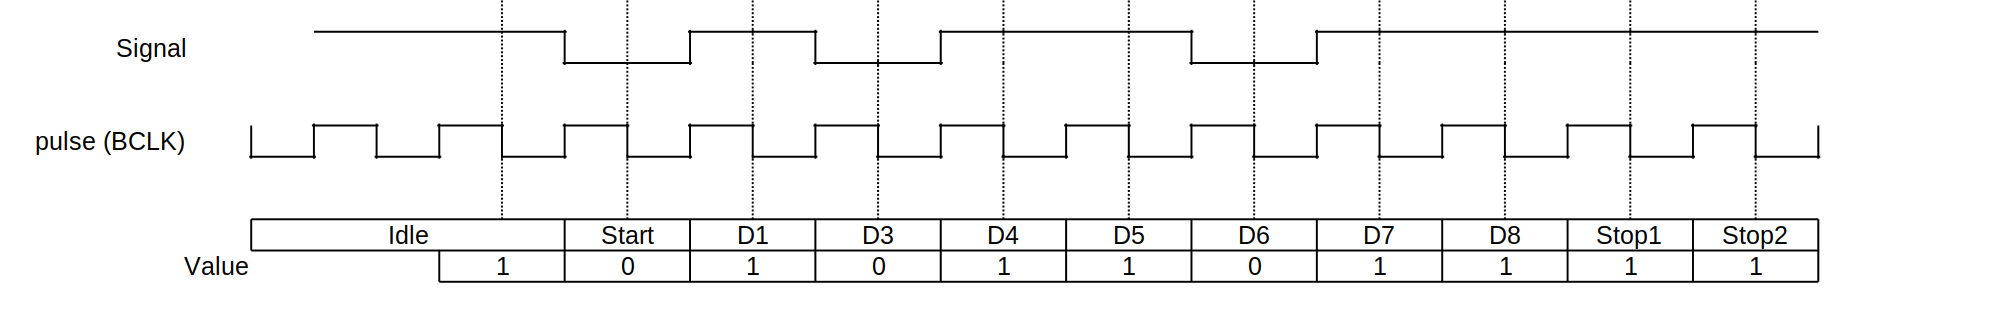
\includegraphics[width=0.9\linewidth]{media/UART.png}
        \caption{By EidenNor - Own work, CC BY-SA 4.0, https://commons.wikimedia.org/w/index.php?curid=118379174}
    \end{figure}
\end{frame}

\begin{frame}
    \frametitle{Transmission of Data Bits}
    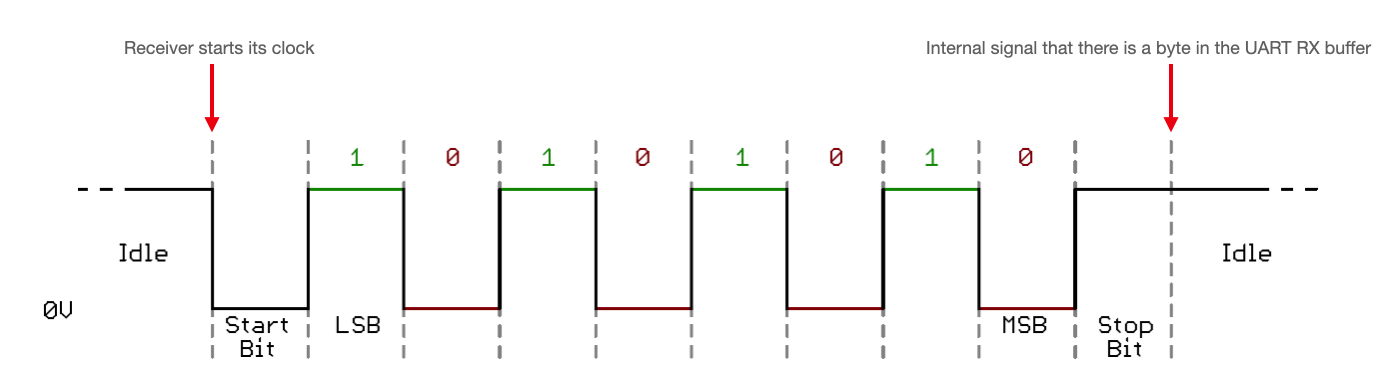
\includegraphics[width=0.8\linewidth]{media/uart_timing.png}
\end{frame}


% \begin{frame}
%     \frametitle{Exam Question}
%     Template: Having the X UART configuration, what is the maxim data rate that can be achieved?

%     Example: Having the 3.3V 9600 baud rate 8E1 with no flow control UART configuration, what is the maxim data rate that can be achieved?
% \end{frame}